\documentclass[11pt]{article}
\usepackage{euscript}

\usepackage{amsmath}
\usepackage{amsthm}
\usepackage{amssymb}
\usepackage{epsfig}
\usepackage{xspace}
\usepackage{color}
\usepackage{url}
\usepackage{subfig}
\usepackage{float}
\usepackage{array}
\graphicspath{ {images/} }
%%%%%%%  For drawing trees  %%%%%%%%%
\usepackage{tikz}
\usetikzlibrary{calc, shapes, backgrounds}

%%%%%%%%%%%%%%%%%%%%%%%%%%%%%%%%%
\setlength{\textheight}{9in}
\setlength{\topmargin}{-0.600in}
\setlength{\headheight}{0.2in}
\setlength{\headsep}{0.250in}
\setlength{\footskip}{0.5in}
\flushbottom
\setlength{\textwidth}{6.5in}
\setlength{\oddsidemargin}{0in}
\setlength{\evensidemargin}{0in}
\setlength{\columnsep}{2pc}
\setlength{\parindent}{1em}
%%%%%%%%%%%%%%%%%%%%%%%%%%%%%%%%%


\newcommand{\eps}{\varepsilon}

\renewcommand{\c}[1]{\ensuremath{\EuScript{#1}}}
\renewcommand{\b}[1]{\ensuremath{\mathbb{#1}}}
\newcommand{\s}[1]{\textsf{#1}}
\newcommand{\tb}[1]{\textbf{#1}}

\newcommand{\E}{\textbf{\textsf{E}}}
\renewcommand{\Pr}{\textbf{\textsf{Pr}}}
\newcommand*{\escape}[1]{\texttt{\textbackslash#1}}


\title{\textbf{\underline{Asmt 2: Document Similarity and  Hashing}}}
%\footnote{\s{CS 6140  Data Mining; \;\; Spring 2015 \hfill
%Instructor: Jeff M. Phillips, University of Utah}
%}

\author{Anirudh Narasimhamurthy(u0941400)}

\begin{document}
\maketitle

\section{Creating \emph k-Grams}

\begin{itemize}
	
	
	\item[] In this part of the question I constructed k-grams for the given documents based on both characters and words. For the k-grams based on characters, 27 characters i.e 26 lower cased alphabets plus space was considered. In the initial copy of the documents, doc1 had a '-' and it also had \escape{r} and \escape{n} characters. I had handled them in my python script but I realized the documents were cleaned and the latest version does not have other characters apart from space and alphabets. For the k-grams based on words space was considered as the delimiter between the words and I had stored the list of all words in a list and then found out the k-grams for the individual documents.
	
	\item[] \textbf{Part A}

	\textbf{Distinct \emph{k}-Grams}

	For storing the k-grams of all the documents, I had made use of the set data structure in python. It also ensures that whenever an addition is made to the set, it only adds distinct elements and hence duplicates are handled and would not be able to enter. The list of distinct k-grams for both characters and words for all the 4 documents have been tabulated below:

	\begin{table}[h]
		\centering
		\begin{tabular}{|c|c|c|c|c|}
			\hline
			\textbf{k-Grams}  & \textbf{Doc1} & \textbf{Doc2} & \textbf{Doc3} & \textbf{Doc4}  \\
			\hline
			\textbf{2-grams characters} &  337   &  378     &  267     &  298  \\
			\hline
			\textbf{3-grams characters} &  1330    &  1590     &  853     &  1074     \\
			\hline
			\textbf{3-grams words}  &  1021    &  1027    &  353    &  505    \\
			\hline
		\end{tabular}
		\caption{Distinct k-grams for each document}
		\label{t2}
	\end{table}
	
	These are the 12 different numbers which we had been asked to report for this part of the question.
	
	\item[] \textbf{Part B}
	
	\textbf{ Jaccard Similarity}
	
	Once the k-grams for all the documents was computed, calculating the Jaccard Similarity was a straight forward implementation. All the k-grams for the four different documents were stored in the sets and so the Jaccard Similarity between any two pairs of documents was computed using the following formula:
	\begin{center}
	$JS(A,B)=\frac{| A \cap  B|}{|A \cup B|}$
	\end{center}

	

	In our case A and B might refer to Doc1, Doc2 or Doc2,Doc3 or Doc3,Doc4 and so on. 
	
	Programmatically this translates to finding the set of all k-grams common to two docuements and the total set of distinct k-grams in both documents. Python has built in methods for finding the union and intersection of two sets. Though it has  built-in methods, I had coded the logic for union and intersection and used that in my program.
	
	
	The Jaccard similarity was computed for the different pairs of documents and the results have been tabulated below:


	\begin{table}[h]
		\centering
		\begin{tabular}{|c|c|c|c|c|}
			\hline
			\textbf{Jaccard Similarity}  & \textbf{Doc1} & \textbf{Doc2} & \textbf{Doc3} & \textbf{Doc4}  \\
			\hline
			Document 1&    &  \textbf{0.8523}   &  \textbf{0.7207}     &  \textbf{0.7255}  \\
			\hline
			Document 2 &      &      &  \textbf{0.6623}    &  \textbf{0.6984}    \\
			\hline
			Document 3 &      &     &     &  \textbf{0.7121}    \\
			\hline
		\end{tabular}
		\caption{Jaccard similarity for all document pairs for 2-grams characters}
		\label{t2}
	\end{table}
	
	The Jaccard Similarity between the same documents would always be 1 and hence the diagnol entries for (Document1,Doc1), (Document2, Doc2) and (Document3,Doc3) are always 1. If we were to think in terms of sets these would be singleton sets and hence the union or the intersection would yield the set itself. This is not asked in the question. But I just wanted make my results clear for the grader. 
	
	Also JS(A,B)=JS(B,A) as per the definition. Hence the values for (Document2,Doc1), (Document3,Doc1) and (Document3, Doc2) have been left blank as they have already been computed and tabulated in (Document1,Doc2),(Document1, Doc3) and (Document2, Doc3) respectively
	
	\begin{table}[h]
		\centering
		\begin{tabular}{|c|c|c|c|c|}
			\hline
			\textbf{Jaccard Similarity}  & \textbf{Doc1} & \textbf{Doc2} & \textbf{Doc3} & \textbf{Doc4}  \\
			\hline
			Document 1&    &  \textbf{0.6957}   &  \textbf{0.4631}     &  \textbf{0.3984}  \\
			\hline
			Document 2&      &      &  \textbf{0.3864}    &  \textbf{0.3529}    \\
			\hline
			Document 3&      &     &    &  \textbf{0.3522}   \\
			\hline
		\end{tabular}
		\caption{Jaccard similarity for all document pairs for  3-grams characters}
		\label{t2}
	\end{table}
	

	
	\begin{table}[h]
		\centering
		\begin{tabular}{|c|c|c|c|c|}
			\hline
		\textbf{Jaccard Similarity}  & \textbf{Doc1} & \textbf{Doc2} & \textbf{Doc3} & \textbf{Doc4}  \\
		\hline
			Document 1 &   &  \textbf{0.3617}   & \textbf{ 0.04169 }    &  \textbf{0.00065}  \\
			\hline
			Document 2 &      &      &  \textbf{0.016949}    &  \textbf{0.000653}    \\
			\hline
			Document 3 &      &     &    &  \textbf{0.001166}  \\
			\hline
		\end{tabular}
		\caption{Jaccard similarity for all document pairs for  3-grams words}
		\label{t2}
	\end{table}
	
		There are six values in each of the three tables above which have been highlighted in bold font. These are the required 18 numbers to be reported for this question.
		
		So this was the expalantion for how I had gone about computing the values which were asked to be reported for Question 1.
	
	\pagebreak
	\end{itemize}




	
\section{Min Hashing}

\begin{itemize}
\item[] \textbf{Part A} 

\textbf{Building MinHash signature and calculating Jaccard Similarity}

In this part of the assignment, we are asked to build a min-hash signature for the documents D1 and D2 using 3-grams based on characters. This process has to be done with  different values of t=\{10,50,100,250,500\} hash functions. For each of the different values of we are also asked to report the Jaccard Similarity between the pair of documents.

Approximate Jaccard Similarity between the pair of documents D1 and D2 is given by:

\begin{center}
$JS_t(a,b) = \frac{1}{t} \cdot \sum _{i=1}^{t}
\begin{cases}
1 & \text{if } a_i=b_i\\
0,& \text{if 
	} a_i \neq b_i\\
\end{cases}$
\end{center}

\textbf{ Methodology Used:}
\begin{itemize}
	

\item To generate the different hash functions I made use of SHA1 hash function available in python. By default, the SHA1 hash function works only on strings and not on integers or floats. I had initially applied it to all the k-grams in Doc1 to check the values it was returning. I made use of the hexdigest() attribute to return the value

\item The function was returning hexadecimal values and size of the resulting hash was 20 bytes. In other words the hash returned by the function comprised of 40 characters each of which is 4 bits.

\item Since we are using min hashing, the signature for the document consists of a vector which has the  minimum value among all the values returned by the particular hash function for all the k-grams in the document. Thus when we use t=5 hash functions our signature will be 5 x1 or 1 x 5 vector.

\item If the corresponding values in the signatures of D1 and D2 match, then we give it a value of 1, else we give it 0. In other words if the first element of D1's signature is 1 and the first element of D2's signature is also 1, then we would give a value of 1 and compute the Jaccard Similarity as per the expression mentioned above.

\item One more important point to be mentioned is that the different hash functions like t=100,250 and 500 were generated by encoding  a salt with sha1. Salt was generated randomly and hence this would ensure that we pick a random hash function h from the hash family. 

\end{itemize}
The approximate Jaccard similarity between the pairs of documents D1 and D2 were calculated and results have been tabulated below. 


	\begin{table}[h]
		\centering
		\begin{tabular}{|c|c|}
			\hline
			\textbf{t} & \textbf{JS(D1,D2)}   \\
			\hline
			10 &  0.6 \\
			\hline
			50 &    0.72    \\
			\hline
			100 &   0.71    \\
			\hline
			250 &    0.688   \\
			\hline
			500 &  0.672     \\
			\hline
		\end{tabular}
		\caption{Jaccard similarity for D1 and D2 based on min-hash signature }
		\label{t2}
	\end{table}
	
	
 
\item[] \textbf{Part B}
 
 To determine good value of t, we could take different approaches and provide a justification for our answer. As mentioned by \textbf{ Anusha (TA) } in the class forum, I would like to provide the justification in terms of the running time and the value computed and its closeness to the actual Jaccard Similarity.
 
 The time taken by the different hash functions {t=10,50,100,250,500} along with their Jaccard similarity computed via MinHashing signature is tabulated below:
 
 \begin{table}[h]
 	\centering
 	\begin{tabular}{|c|c|c|}
 		\hline
 		\textbf{t} & \textbf{JS(D1,D2)}  & Running time(in seconds) \\
 		\hline
 		10 &  0.6 &  0.0835\\
 		\hline
 		50 &    0.66 &  0.46788  \\
 		\hline
 		100 &   0.70  &  0.946 \\
 		\hline
 		250 &    0.688 &  2.3527\\
 		\hline
 		500 &  0.674 & 4.5416\\
 		\hline
 		1000 &  0.687 & 9.7218\\
 		\hline
 	\end{tabular}
 	\caption{Jaccard similarity for D1 and D2 based on min-hash signature }
 	\label{t2}
 \end{table}
 
 
 A point to be mentioned. This time was taken or considered only for the lines of code that are  computing the Jaccard similarity via the Min Hash signature and not for the entire program.
 
 I also experimented with t=1000 and have tabulated the results. From the experiments, I found that a good value of t from the given values would be \textbf{t=100}. The reasons are provided below:
 
 \begin{itemize}
 	\item The actual Jaccard Similarity between D1 and D2 is 0.6957 and the Jaccard Similarity obtained via minhashing signature for t=100 is 0.7 which is very close to the actual value.
 	
 	\item Although t=200 or t=500 would definitely be better considering they are doing several times more and taking an average out of that for Jaccard Similarity. But the problem as we see is the time taken for computing increases  as 't' increases.
 	
 	\item The documents provided in the assignment were relatively small by any standards and so for this experiment, it might not seem to be a bad idea to pick t as say 200, but when min hashing is generally applied to large documents the execution time overhead might be there with respect to t=250 and t=500.
 	
 	\item One thing which was clear as to why we shouldn't choose a smaler value of \emph{t} say like 10. This is because 10  iterations is really small and the simlarities computed using it might be way off either on the upside or on the downside.
 	
 	\item Hence t=100 is a good value which satisifes both our accuracy and time constraints. If we were allowed to take/choose an arbitrary value of \emph{t} for the given documents, I feel a value in the range of 150-180 would be really ideal for the given pair of documents. \\
 \end{itemize}
 
 
\end{itemize}
\pagebreak

\section{LSH}

\begin{itemize}
	\item[] \textbf{Part A}
	
	We are asked to report the best values of b and r for this question. Here r is the number of bands and b is the number of hashes per band.
	
	Based on the information provided in the notes, we know that given the budget of the number of hash functions \emph t and the threshold value of $\tau$, the value of b can be approximately estimated using the following expression:
	
	\begin{center}
		$b \approx - log_{\tau}(t)$
	\end{center}
	
	Plugging in the value of \emph t as 100 and $\tau$ as 0.4 we get,
		\begin{itemize}
		\item[] $b \approx - log_{0.4}(100)$
		\item[]  $b \approx 5.02588$
		\item[] $\boxed{ b= 5}$
		\end{itemize}
		
	The budget on the number of hash functions \emph t is split/divided into r and b. Now that we have obtained the value of b in the previous step, we can obtain \emph r using the following formula:
	\begin{itemize}
		\item[] t= b. r
		\item[] r= t/b
		\item[] r=100/5
		\item[] \boxed{r=20}
	\end{itemize}	
	
	We can verify if these values of t and r provide us an S-curve where on the x-axis we could have the JS(D1,D2) between the documents represented and the y-axis representing the probability that the pair $D1,D2$ is a candidate to check the true distance.
	
	Using the expression we can find the values needed for the plot \begin{center}
		$f(s)=1-(1-s^{b})^{r}$
	\end{center}
	
	In our case r=20 and b=5.\\
	
	\begin{itemize}
		\item[] $f(0.1)=0.0001$
		\item[] $f(0.2)=0.0063$
		\item[] $f(0.3)=0.0474$
		\item[] $f(0.4)=0.1860$
		\item[] $f(0.5)=0.4700$
		\item[] $f(0.6)=0.80190$
		\item[] $f(0.7)=0.9747$
		\item[] $f(0.8)=0.9964$
		\item[] $f(0.9)=0.9999$
		
	\end{itemize}
	
	\begin{figure}[H]%
		\centering
		\subfloat[Probability that distance d(D1,D2) is checked in a LSH scheme with r=20 bands and b=5 hahses each]{{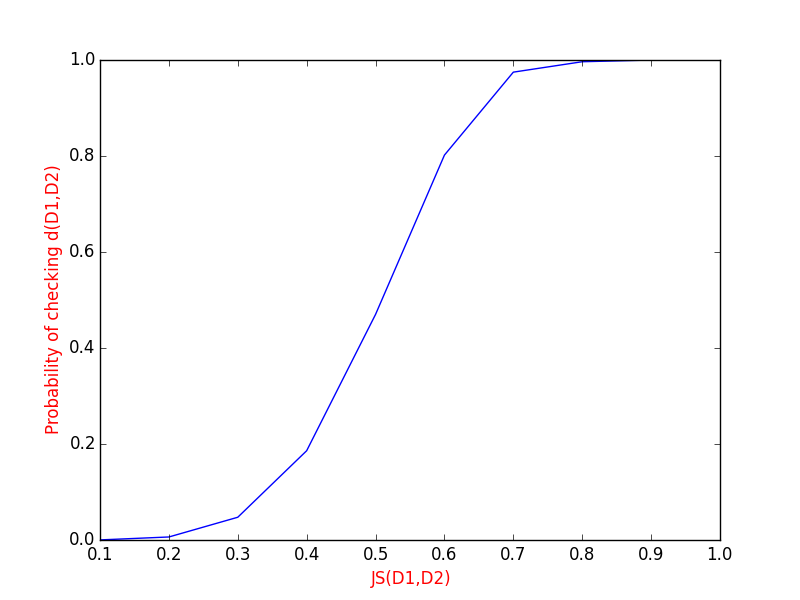
\includegraphics[width=7cm]{LSH_plot} }}%
		
	\end{figure}
	
	
	
	These are the values which were required to be reported for this question.	
\item[] \textbf{Part B}

In this part we are asked to find what is the probability that each of pair of four documents will be estimated to have a similarity greater than $\tau$

There are two possible explanations for the selection of Jaccard similarity for this question. The text book considers s as the Jaccard similarity which was computed via min hashing, while Professor's notes have s=JS(D1,D2) which was computed in problem 1. 

I personally feel given that we have the Jaccard similarity of the pairs of  documents which gives us very accurate value, using the approximate value of Jaccard Similarity computed using Min-hashing isn't entirely convinving. But I have decided to show the work for both the appoaches. the calculations are done below:


\textbf{If we consider the s= Approximate Jaccard Similarity computed via Min Hashing}

 We have also computed the values of b and r in the previous part. Now we would have to plug in those values in the expression below:

\begin{center}
$f(s)=1-(1-s^{b})^{r}$
\end{center}

Here f(s) relates to the probability LSH, with our choice of r and b will classify it as being above tau. 

\textbf{For Document1 and Document 2}
\begin{itemize}
	\item[] $f(s)=1-(1-s^{b})^{r}$
	\item[] $f(s)=1-(1-0.71^{5})^{20}$
	\item[] $\boxed{f(s)=0.9813}$
\end{itemize}

\textbf{For Document1 and Document 3}
\begin{itemize}
	\item[] $f(s)=1-(1-s^{b})^{r}$
	\item[] $f(s)=1-(1-0.42^{5})^{20}$
	\item[] $\boxed{f(s)=0.23133}$\\
\end{itemize}

\textbf{For Document1 and Document 4}
\begin{itemize}
	\item[] $f(s)=1-(1-s^{b})^{r}$
	\item[] $f(s)=1-(1-0.38^{5})^{20}$
	\item[] $\boxed{f(s)=0.14709}$\\
\end{itemize}

\textbf{For Document2 and Document 3}
\begin{itemize}
	\item[] $f(s)=1-(1-s^{b})^{r}$
	\item[] $f(s)=1-(1-0.41^{5})^{20}$
	\item[] $\boxed{f(s)=0.20789}$\\
\end{itemize}



\textbf{For Document2 and Document 4}
\begin{itemize}
	\item[] $f(s)=1-(1-s^{b})^{r}$
	\item[] $f(s)=1-(1-0.32^{5})^{20}$
	\item[] $\boxed{f(s)=0.0650}$\\
\end{itemize}

\textbf{For Document3 and Document 4}
\begin{itemize}
	\item[] $f(s)=1-(1-s^{b})^{r}$
	\item[] $f(s)=1-(1-0.37^{5})^{20}$
	\item[] $\boxed{f(s)=0.1299}$\\
\end{itemize}



\begin{table}[h]
	\centering
	\begin{tabular}{|c|c|c|c|c|}
		\hline
		\textbf{Probability that docs have similarity  $ > \tau$}  & \textbf{Doc1} & \textbf{Doc2} & \textbf{Doc3} & \textbf{Doc4}  \\
		\hline
		Document 1&    &  \textbf{0.9813}   &  \textbf{0.23133}     &  \textbf{0.14709}  \\
		\hline
		Document 2&      &      &  \textbf{0.20789}    &  \textbf{0.0650}    \\
		\hline
		Document 3&      &     &    &  \textbf{0.1299}   \\
		\hline
	\end{tabular}
	\caption{Probability that each pair of documents will have similarity $ > \tau $}
	\label{t2}
\end{table}


\textbf{ If we consider s= Jaccard Similarity between the pairs of Documents}

\textbf{For Document1 and Document 2}
\begin{itemize}
	\item[] $f(s)=1-(1-s^{b})^{r}$
	\item[] $f(s)=1-(1-0.6957^{5})^{20}$
	\item[] $\boxed{f(s)=0.9715}$
\end{itemize}

\textbf{For Document1 and Document 3}
\begin{itemize}
	\item[] $f(s)=1-(1-s^{b})^{r}$
	\item[] $f(s)=1-(1-0.4631^{5})^{20}$
	\item[] $\boxed{f(s)=0.3498}$\\
\end{itemize}

\textbf{For Document1 and Document 4}
\begin{itemize}
	\item[] $f(s)=1-(1-s^{b})^{r}$
	\item[] $f(s)=1-(1-0.3984^{5})^{20}$
	\item[] $\boxed{f(s)=0.1827}$\\
\end{itemize}

\textbf{For Document2 and Document 3}
\begin{itemize}
	\item[] $f(s)=1-(1-s^{b})^{r}$
	\item[] $f(s)=1-(1-0.3864^{5})^{20}$
	\item[] $\boxed{f(s)=0.1588}$\\
\end{itemize}



\textbf{For Document2 and Document 4}
\begin{itemize}
	\item[] $f(s)=1-(1-s^{b})^{r}$
	\item[] $f(s)=1-(1-0.3529^{5})^{20}$
	\item[] $\boxed{f(s)=0.1039}$\\
\end{itemize}

\textbf{For Document3 and Document 4}
\begin{itemize}
	\item[] $f(s)=1-(1-s^{b})^{r}$
	\item[] $f(s)=1-(1-0.3522^{5})^{20}$
	\item[] $\boxed{f(s)=0.1029}$\\
\end{itemize}



\begin{table}[h]
	\centering
	\begin{tabular}{|c|c|c|c|c|}
		\hline
		\textbf{Probability that docs have similarity  $ > \tau$}  & \textbf{Doc1} & \textbf{Doc2} & \textbf{Doc3} & \textbf{Doc4}  \\
		\hline
		Document 1&    &  \textbf{0.9715}   &  \textbf{0.3498}     &  \textbf{0.1827}  \\
		\hline
		Document 2&      &      &  \textbf{0.1588}    &  \textbf{0.1039}    \\
		\hline
		Document 3&      &     &    &  \textbf{0.1029}   \\
		\hline
	\end{tabular}
	\caption{Probability that each pair of documents will have similarity $ > \tau $}
	\label{t2}
\end{table}

These are the 6 required values which needs to be reported for this question.

\end{itemize}


\end{document}
